%\section{A Parallel Pattern Programming Model}
\section{Parallel Patterns}
\label{patterns}

\subsection{Programming with Parallel Patterns}

% \begin{table*}[]
% \centering
% \begin{tabular}{l|cccc}
% \toprule
% & \multicolumn{1}{c}{\bf{Map}} & \bf{Fold}  & \bf{FlatMap} & \bf{HashReduce} \\ \midrule
% &
% \texttt{\footnotesize{Indices}}\vspace{-0.5mm} &
% \texttt{\footnotesize{Indices}}\vspace{-0.5mm} &
% \texttt{\footnotesize{ Indices}}\vspace{-0.5mm} &
% \texttt{\footnotesize{  Indices}}\vspace{-0.5mm} \\

% &
% \belowbaseline[-25pt]{ 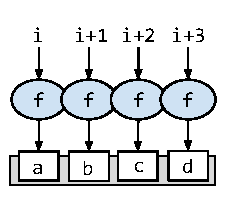
\includegraphics[width=3.0cm]{figs/Map.pdf}  }&
% \belowbaseline[-20pt]{ 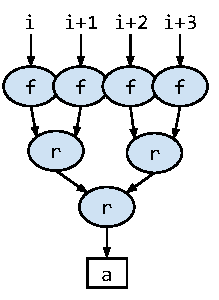
\includegraphics[width=3.0cm]{figs/Reduce.pdf}  }&
% \belowbaseline[-20pt]{ 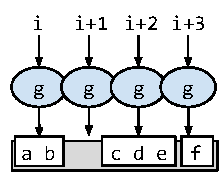
\includegraphics[width=3.0cm]{figs/FlatMap.pdf} }&
% \belowbaseline[-20pt]{ 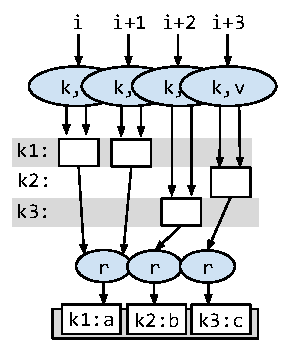
\includegraphics[width=3.9cm]{figs/HashReduce.pdf} }\\
% \midrule

% Compute &
% \multicolumn{4}{c}{\begin{tabular}[c]{@{}c@{}}Pipelined, programmable compute\\ SIMD lanes\end{tabular}} \\
% \midrule

% % On-chip Memory
% \multirow{2}{*}{\begin{tabular}[c]{@{}l@{}}On-Chip\\ Memory\end{tabular}} &
%   \multicolumn{4}{c}{\begin{tabular}[c]{@{}c@{}}Distributed register files (intermediate scalars)\end{tabular}} \\
% & \multicolumn{4}{c}{\begin{tabular}[c]{@{}c@{}}Double buffering support\end{tabular}} \\
% \cline{2-5}

% & \multicolumn{1}{c|}{\begin{tabular}[c]{@{}c@{}}Banked scratchpads\end{tabular}} &
%   \multicolumn{1}{c|}{} &
%   \multicolumn{1}{c|}{\begin{tabular}[c]{@{}c@{}}Banked FIFO\\memories \end{tabular}} &
%   \multicolumn{1}{c}{\begin{tabular}[c]{@{}c@{}}CAM (sparse)\\Banked\\scratchpads (dense)\end{tabular}} \\
% \midrule

% % Off-chip memory
% \multirow{3}{*}{\begin{tabular}[c]{@{}l@{}}Off-Chip\\ Memory\end{tabular}} &
%   \multicolumn{4}{c}{\begin{tabular}[c]{@{}c@{}}Burst commands (linear reads and writes)\end{tabular}} \\ %\cline{2-5}
% & \multicolumn{4}{c}{\begin{tabular}[c]{@{}c@{}}Gather support (random reads)\end{tabular}} \\ %\cline{2-5}
% & \multicolumn{4}{c}{\begin{tabular}[c]{@{}c@{}}Scatter support (random writes)\end{tabular}} \\ %\cline{2-5}
% %& \multicolumn{4}{c}{\begin{tabular}[c]{@{}c@{}}Address coalescing to minimize DRAM requests\end{tabular}} \\ %\cline{2-5}
% %& \multicolumn{4}{c}{\begin{tabular}[c]{@{}c@{}}Multiple outstanding memory requests to utilize memory bandwidth\end{tabular}} \\
% \midrule

% %Interconnect
% \multirow{1}{*}{\begin{tabular}[c]{@{}l@{}}Interconnect\end{tabular}} &
% \multicolumn{1}{c|}{} &
% \multicolumn{1}{c|}{Cross-lane reduction tree}&
% \multicolumn{1}{c|}{Cross-lane coalescing} &
% \multicolumn{1}{c}{} \\
% \midrule

% %Control
% \multirow{2}{*}{\begin{tabular}[c]{@{}l@{}}Control\end{tabular}} &
%   \multicolumn{4}{c}{\begin{tabular}[c]{@{}c@{}}Parallelizable counter chains for generating indices\end{tabular}} \\ %\cline{2-5}
% & \multicolumn{4}{c}{\begin{tabular}[c]{@{}c@{}}Reconfigurable control for hierarchical pipelining\end{tabular}} \\

% \bottomrule
% \end{tabular}

% \caption{The parallel patterns and their corresponding hardware implementation requirements}
% \label{t:patterns}
% \end{table*}


Parallel patterns are an extension to traditional functional programming which capture parallelizable computation on both dense and sparse data collections along with corresponding memory access patterns.
Parallel patterns enable simple, automatic program parallelization rules for common computation tasks
while also improving programmer productivity through higher level abstractions.
The performance benefit from parallelization, coupled with improved programmer productivity, has caused parallel patterns to become increasingly popular in a variety of domains,
including machine learning, graph processing, and database analytics~\cite{ecoop13sujeeth,pldi13halide}.
Previous work has shown how parallel patterns can be used in functional programming models to generate multi-threaded
C++ for CPUs comparable to hand optimized code~\cite{delite-tecs14} and efficient accelerator designs for FPGAs~\cite{auerbach10lime,george14fpl,delite2maxj}.
As with FPGAs and multi-core CPUs, knowledge of data parallelism is vital to achieve good performance when targeting CGRAs.
This implicit knowledge makes parallel patterns a natural programming model to drive CGRA design.

Like previous work on hardware generation from parallel patterns~\cite{george14fpl,delite2maxj}, our programming model is based on 
the parallel patterns \emph{Map}, \emph{FlatMap}, \emph{Fold}, and \emph{HashReduce}. These patterns are selected because they are most amenable to hardware acceleration.
Table~\ref{t:patterns} depicts conceptual examples of each pattern, where computation is shown operating on four indices simultaneously.
Every pattern takes as input one or more functions and an \emph{index domain} describing the range of values that the pattern operates over.
Each of these patterns builds an output and reads from an arbitrary number of input collections.


\emph{Map} creates a single output element per index using the function \emph{f}, where each execution of \emph{f} is guaranteed to be independent.
The number of output elements from Map is the same as the size of the input iteration domain.
Based on the number of collections read in \emph{f} and the access patterns of each read, Map can capture the behavior of a gather, a standard element-wise map, a zip, a windowed filter, or any combination thereof.

\emph{FlatMap} produces an arbitrary number of elements per index using function \emph{g}, where again function execution is independent. The produced elements are concatenated into a flat output. Conditional data selection (e.g. \emph{WHERE} in SQL, \emph{filter} in Haskell or Scala) is a special case of FlatMap where \emph{g} produces zero or one elements.

\emph{Fold} first acts as a Map, producing a single element per index using the function \emph{f}, then reduces these elements using an associative combine function \emph{r}.

\emph{HashReduce} generates a hash key and a value for every index using functions \emph{k} and \emph{v}, respectively. Values with the same corresponding key are reduced on the fly into a single accumulator using an associative combine function \emph{r}. HashReduce may either be dense, where the space of keys is known ahead of time and all accumulators can be statically allocated, or sparse, where the pattern may generate an arbitrary number of keys at runtime. Histogram creation is a common, simple example of HashReduce where the \emph{key} function gives the histogram bin, the \emph{value} function is defined to always be "1", and the \emph{combine} function is integer addition.

    %// (*@\emph{\textbf{Outer Map function (f1)}} @*) 
      %// (*@\emph{\textbf{Inner map function (f2)}} @*) 
      %// (*@\emph{\textbf{Combine function (r)}} @*)
\begin{figure}\centering
\begin{lstlisting}[language=Scala]
val a: Matrix[Float]  // M x N
val b: Matrix[Float]  // N x P
val c = Map(M, P){(i,j) =>
  // Outer Map function (f1)
  Fold(N)(0.0f){k =>
    // Inner map function (f2)
    a(i,k) * b(k,j)
  }{(x,y) =>
    // Combine function (r)
    x + y
  }
}
\end{lstlisting}
\vspace{-10pt}
\caption{Example of using Map and Fold in a Scala-based language for computing an untiled matrix multiplication using inner products. }
\label{fig:matmult}
%\vspace{-10pt}
\end{figure}

  %// (*@\emph{\textbf{Key function (k)}} @*)
  %// (*@\emph{\textbf{Value function (v)}} @*)
  %// (*@\emph{\textbf{Combine function (r) - combine using summation}} @*)
\begin{figure}\centering
\begin{lstlisting}[language=Scala]
val CUTOFF: Int = Date("1998-12-01")
val lineItems: Array[LineItem] = ...
val before = lineItems.filter{ item => item.date < CUTOFF }

val query = before.hashReduce{ item =>
  // Key function (k)
  (item.returnFlag, item.lineStatus)
}{ item =>
  // Value function (v)
  val quantity = item.quantity
  val price = item.extendedPrice
  val discount = item.discount
  val discountPrice = price * (1.0 - discount)
  val charge = price * (1.0 - discount) * (1.0 + item.tax)
  val count = 1
  (quantity, price, discount, discountedPrice, count)
}{ (a,b) =>
  // Combine function (r) - combine using summation
  val quantity = a.quantity + b.quantity
  val price = a.price + b.price
  val discount = a.discount + b.discount
  val discountPrice = a.discountPrice + b.discountPrice
  val count = a.count + b.count
  (quantity, price, discount, discountPrice, count)
}
\end{lstlisting}
\vspace{-10pt}
\caption{Example of using filter (FlatMap) and HashReduce in a Scala-based language, inspired by TPC-H query 1. }
\label{fig:tpchq1}
\vspace{-5pt}
\end{figure}

%%% Code example explanation
Figure~\ref{fig:matmult} shows an example of writing an untiled matrix
multiplication with an explicit parallel pattern creation syntax. In
this case, the Map creates an output matrix of size \texttt{M}~$\times$~\texttt{P}. 
The Fold produces each element of this matrix using a dot product over \texttt{N} elements.
Fold's map function (\texttt{f2}) accesses an element of matrix \texttt{a} and matrix \texttt{b} and multiplies them.
Fold's combine function (\texttt{r}) defines how to combine arbitrary elements produced by \texttt{f2}, in this case using summation.


Figure~\ref{fig:tpchq1} gives an example of using parallel patterns in a Scala-based language, where infix operators have been
defined on collections which correspond to instantiations of parallel patterns. Note that in this example, the \texttt{filter} on line 3 creates
a FlatMap with an index domain equal to the size of the \texttt{lineItems} collection. The \texttt{hashReduce} on line 5 creates a HashReduce with an index domain with the size of the \texttt{before} collection.



%\christos{For the memory patterns, I'd say
%  bank scratchpad (X) where X is the access pattern (FIFO, etc). The
%  off-chip memory entry is confusing as it does not say which pattern
%  uses which feature}\christos{You can trim 2.1 if needed}


\subsection{Hardware Implementation Requirements}
Parallel patterns provide a concise set of parallel abstractions that can succinctly express a wide variety of 
machine learning and data analytic algorithms \cite{ecoop13sujeeth, pldi13halide, catanzaro11copperhead, delite2maxj}.
By creating an architecture with specialized support for these patterns, we can execute these algorithms efficiently.
This parallel pattern architecture requires several key hardware features, described below and summarized in Table~\ref{t:requirements}.

%We would like our reconfigurable hardware accelerator to be able to take advantage of the high level programming and compiler information granted by parallel patterns.
%To most efficiently support these patterns, the hardware should have a variety of architectural features, summarized in Table~\ref{t:patterns}.

\begin{table}[]
\centering
\resizebox{0.95\columnwidth}{!}{%
\begin{tabular}{rcc}
\toprule
{} & \small{\textbf{Programming Model}} & \small{\textbf{Hardware}} \\
\midrule

\footnotesize

\multirow{2}{*}{\begin{tabular}[c]{@{}l@{}}\small{\textbf{Compute}}\end{tabular}} &
\multirow{2}{*}{\begin{tabular}[c]{@{}c@{}}\small{Parallel patterns}\end{tabular}} &
\small{Pipelined compute} \\
& &{\begin{tabular}[c]{@{}c@{}}\small{SIMD lanes}\end{tabular}} \\
\midrule

\multirow{5}{*}{\begin{tabular}[c]{@{}l@{}}\small{\textbf{On-Chip}}\\ \small{\textbf{Memory}}\end{tabular}} &
     \small{Intermediate scalars} & \small{Distributed pipeline registers} \\
{} & \small{Tiled, linear accesses} & \small{Banked scratchpads} \\
{} & \small{Random reads} & \small{Duplicated scratchpads} \\
{} & \small{Streaming, linear accesses} & \small{Banked FIFOs} \\
{} & \small{Nested patterns} & \small{Double buffering support} \\
\midrule

\multirow{2}{*}{\begin{tabular}[c]{@{}l@{}}\small{\textbf{Off-Chip}}\\\small{\textbf{Memory}}\end{tabular}} &
  \small{Linear accesses} & \small{Burst commands} \\
{} & \small{Random reads/writes}  & \small{Gather/scatter support} \\
%{} & \small{Random writes} & \small{Scatter support} \\
\midrule

\multirow{2}{*}{\begin{tabular}[c]{@{}l@{}}\small{\textbf{Interconnect}}\end{tabular}} &
     \small{Fold}    & \small{Cross-lane reduction trees} \\
{} & \small{FlatMap} & \small{Cross-lane coalescing} \\
\midrule

\multirow{2}{*}{\begin{tabular}[c]{@{}l@{}}\small{\textbf{Control}}\end{tabular}} &
     \small{Pattern indices} & \small{Parallelizable counter chains} \\
{} & \small{Nested patterns} & \small{Programmable control} \\
\bottomrule
\end{tabular}
}

\caption{Programming model components and their corresponding hardware implementation requirements.}
\label{t:requirements}
\vspace{-20pt}
\end{table}

First, all four patterns express data-parallel computation where operations on each index are entirely independent.
An architecture with pipelined compute organized into SIMD lanes exploits this data parallelism to achieve a multi-element per cycle throughput.
Additionally, apart from the lack of loop-carried dependencies, we see that functions \emph{f}, \emph{g}, \emph{k}, and \emph{v} in Table~\ref{t:patterns} are otherwise unrestricted.
This means that the architecture's pipelined compute must be programmable in order to implement these functions.

Next, in order to make use of the high throughput available with pipelined SIMD lanes, the architecture must be able to deliver high on-chip memory bandwidth.
In our programming model, intermediate values used within a function are typically scalars with statically known bit widths.
These scalar values can be stored in small, distributed pipeline registers.

Collections are used to communicate data between parallel patterns.
Architectural support for these collections depends on their associated memory access patterns, determined by analyzing the function used to compute the memory's address.
For simplicity, we categorize access patterns as either statically predictable \emph{linear} functions of the pattern indices or unpredictable, \emph{random} accesses.
Additionally, we label accesses as either \emph{streaming}, where no data reuse occurs across a statically determinable number of function executions, or \emph{tiled}, where reuse may occur.
We use domain knowledge and compiler heuristics to determine if a random access may exhibit reuse.
Previous work has shown how to tile parallel patterns to introduce statically sized windows of reuse into the application and potentially increase data locality \cite{delite2maxj}.

%Tiling computation with parallel patterns has previously been shown to improve the number of accesses
%Previous work has also shown how to tile parallel patterns to break up computation into fixed size units and increase the number of accesses with reuse.\cite{delite2maxj}.

Collections with tiled accesses can be stored in local scratchpads.
To drive SIMD computation, these scratchpads should support multiple parallel address streams when possible.
In the case of linear accesses, address streams can be created by banking.
Parallel random reads can be supported by local memory duplication, while random write commands must be sequentialized and coalesced.

Although streaming accesses inevitably require going to main memory, the cost of main memory reads and writes can be minimized by coalescing memory commands and prefetching
data with linear accesses. Local FIFOs in the architecture provide backing storage for both of these optimizations.

%However, local memories can help to store intermediate values to reduce the total number of expensive off-chip accesses.

%Note that for hardware, the distinction of statically known number of executions is important, as this directly corresponds to the size





%%Previous work has shown how to tile parallel patterns to potentially improve locality .
%Collections with streaming accesses can be implemented in the architecture as FIFOs.




%In many algorithms, the patterns can also be tiled

%If the address range is known to be small, memories with linear and random accesses can be implemented as scratchpads.
%A dense HashReduce, for example, exhibits random writes to its output collection, but often within a small, statically known address size.
%Additionally, computation can often be reorganized to work
%Otherwise, caches or content-addressable memories (CAMs) are necessary to store local copies of data.

These local memories allow us to exploit locality
in the application in order to minimize the number of costly loads or
stores to main memory \cite{dark}. Reconfigurable banking support within these
local memories increases the bandwidth available from these on-chip
memories, thus allowing better utilization of the compute. Double
buffering, generalized as \emph{N}-buffering, support in scratchpads
enables coarse-grain pipelined execution of imperfectly nested
patterns.

%In all four parallel patterns, if the output collection is dense, writing to the output collection has a ``sequential'' access pattern.
%Writing to sparse outputs is equivalent to a scatter.

The architecture also requires efficient memory controllers to populate local memories and commit calculated results.
As with on-chip memories, the memory controller should be specialized to different access patterns.
Linear accesses correspond to DRAM burst commands, while random reads and writes in parallel patterns correspond to gathers and scatters, respectively.



%For data structures, the architecture required to achieve high bandwidth depends on the data's memory access patterns.
%Predictable, linear access patterns are common in applications working with dense data structures, while random, data dependent accesses are common for sparse data.
%Dense Map and FlatMap, for example, always have linear writes to their output collections, while sparse Map and HashReduce always write randomly.
%\todo{Linear accesses -> burst access support to main memory} Gather and scatter are also common, especially for sparse data structures, and can be supported in the architecture through dedicated scatter/gather memory control support, command coalescing of random accesses, and support for a large number of outstanding memory requests.

Fold and FlatMap also suggest fine-grained communication across SIMD lanes. Fold requires reduction trees across lanes, while the concatenation in FlatMap is best supported by valid word coalescing hardware across lanes.

Finally, all parallel patterns have one or more associated loop indices. These indices can be implemented in hardware as parallelizable, programmable counter chains.
Since parallel patterns can be arbitrarily nested, the architecture must also have programmable control logic to determine when each pattern is allowed to execute.

While many coarse-grained hardware accelerators have been proposed, no single accelerator described by previous work has all of these hardware features.
This means that, while some of these accelerators can be targeted by parallel patterns, none of them can fully exploit the properties of these patterns to achieve maximum performance.
Traditional FPGAs can also be configured to implement these patterns, but with much poorer energy efficiency, as we show in Section~\ref{evaluation}.
We discuss related work further in Section~\ref{relatedWork}.
%% Finally, have a sentence that it can
  %all be done with a fine-grain FPGA but the overheads are huge as all
%coarse-grain array work has shown.}
